% !Mode:: "TeX:UTF-8"
\documentclass{article}
\usepackage[hyperref, UTF8]{ctex}
\usepackage[dvipsnames]{xcolor}
\usepackage{geometry}
\usepackage{amsmath}
\usepackage{amsfonts}
\usepackage{listings}
\usepackage{pgfplotstable}
\usepackage{pgfplots}
\usepackage{fontspec}
\usepackage{booktabs} % 表格上的不同横线
%\setmainfont{Consolas} %设置英文字体

\definecolor{mygreen}{rgb}{0,0.6,0}
\definecolor{mygray}{rgb}{0.5,0.5,0.5}
\definecolor{mymauve}{rgb}{0.58,0,0.82}
\lstset{ %
    backgroundcolor=\color{white},   % choose the background color
    basicstyle=\footnotesize\ttfamily,        % size of fonts used for the code
    columns=fullflexible,
    breaklines=true,                 % automatic line breaking only at whitespace
    captionpos=b,                    % sets the caption-position to bottom
    tabsize=4,
    backgroundcolor=\color[RGB]{245,245,244},            % 设定背景颜色
    commentstyle=\color{mygreen},    % comment style
    escapeinside={\%*}{*)},          % if you want to add LaTeX within your code
    keywordstyle=\color{blue},       % keyword style
    stringstyle=\color{mymauve}\ttfamily,     % string literal style
    showstringspaces=false,                % 不显示字符串中的空格
    frame=none,
    rulesepcolor=\color{red!20!green!20!blue!20},
    % identifierstyle=\color{red},
    language=c++,
}

% 设置hyperlink的颜色
\newcommand\myshade{85}
\colorlet{mylinkcolor}{violet}
\colorlet{mycitecolor}{YellowOrange}
\colorlet{myurlcolor}{Aquamarine}


\title{软件测试计划}
\author{Tomato}
\date{2018年1月}

\begin{document}

	\maketitle
		\section{引言}
			对于后端我们做了详尽的测试,包括Controller正确性的测试,Service的测试和底层数据库的测试。
			\subsection{系统概述}
				整个test文件包含三种test,分别是Controller的test,Model的test和Service的test。Controller中的test又分为Admin的test和Client的test。由于没有找到微信websocket的test方法,所以微信的websocket没有写test。
			\subsection{文档概述}
				本文档将介绍测试环境,测试计划以及测试进度。
			\subsection{与其他计划的关系}
				测试是在接口实现中逐步完善的。与接口的计划相辅相成,可以说是写一个接口就写了一个test。
		\section{软件测试环境}
			\subsection{后端测试}
				\paragraph{软件项}
					我们所用的语言是Java,使用的框架是Spring Boot,所有的测试都是搭建在这个框架之上的,写测试的方法也是使用了这个框架集成的test annotations。
				\paragraph{参与组织}
					Tomato后端开发组。
				\paragraph{人员}
					张慧盟、宋世虹。
				\paragraph{要执行的测试}
					如上所述,需要测试Controller,Model和Service。
		\section{计划}
			\section{总体设计}
				\subsection{测试过程}
					\subsection{Controller}
						\paragraph{Admin}
							\begin{itemize}
							\item AdminLoginControllerTest: 测试了两种情况,Admin登陆成功和登录失败。
							\item AuctionControllerTest: 测试了Auction的接口,包括当get auction的时候应该返回什么,如果发起了错误的get auction操作时会返回什么,post auction的时候Service的更新, post auction错误的时候返回什么等等。
							\item ChangePasswordControllerTest: 测试了如果password输入正确的更新准则和输入错误时的报错。
							\item CompetitionCreatorControllerTest:测试了创建比赛,更新比赛和获得比赛具体信息时的返回值,以及上述情况request出错时的返回值。
							\item CompetitionInfomationControllerTest:测试了请求比赛信息时返回信息的正确性,和请求失败的返回值。
							\item CompetitionStatusAdminControllerTest:测试了不同比赛状态时的返回值。
							\item DeleteCompetitionControllerTest:测试了删除比赛时:正常删除、没有比赛和获得全部比赛出错的情况。
							\item GetAllCompetitionControllerTest:测试了返回全部比赛时:正常返回、没有比赛、获得全部比赛出错的情况。
							\item UpdateCompetitionStatusControllerTest:测试了更新比赛状态时的返回值:正常返回、没有比赛、后端没法update比赛状态、非法状态等情况。
							\end{itemize}
						\paragraph{Client}
							\begin{itemize}
							\item BuyMaterialControllerTest:测试了买东西时:买材料和买机器的正在交易、已经交易完成和交易取消的情况。
							\item ClientInfoControllerTest:测试了获取和更新team信息时成功和失败时的情况。
							\item ClientLoginControllerTest:测试了登陆成功和失败的情况。
							\item ClientPropertyControllerTest:测试了team获取property时成功、失败的情况,测试了team生产的时候成功和失败的情况,
							\item CompetitionStatusControllerTest:测试了更新比赛状态时Client的返回情况。
							\item GetAllUsersControllerTest:测试了获取所有team的成功和失败的情况。
							\item GetProduceHistoryControllerTest:测试了获取生产历史的成功和失败(没有team,没有produce记录)的情况。
							\item GetTradeHistoryControllerTest:测试了获取交易历史的成功和失败(没有team,没有produce记录)的情况。
							\item ListenPropertyControllerTest:测试了在websocket转发中监听produce后资产的改变。
							\item SellMaterialControllerTest:测试了卖资产时成功的情况,包括各种材料和机器。
							\item SendToSellerControllerTest:测试了将售卖的账单转给买方和卖方的同team,主要测试了不同账单状态的回复情况。
							\item UndoTradeControllerTest:测试了撤销交易的成功情况,主要测试了发给买方和卖方的账单。
							\end{itemize}
					\subsection{Service}
						\begin{itemize}
							\item admin.CompetitionServiceTest: 测试了创建比赛、查找比赛、更新比赛、删除比赛的接口,测试了创建队伍、更新队伍、查找队伍的接口,测试了创建机器、查找机器、更新机器的接口,测试了获得所有Produce信息和交易信息的接口,测试了更新Round的接口。
							\item admin.LoginServiceTest: 测试了创建Admin、更新Admin、查找Admin和删除Admin的接口。
							\item user.CompetitionServiceTest: 测试了查找Competition和更新Competition的成功和失败的情况。
							\item user.LoginServiceTest: 测试了查找team、更新team、创建team和删除team的Service的成功和失败情况。
							\item user.OrderServiceTest: 测试了创建Produce、查找Produce、更新Produce、删除Produce的接口,测试了创建Trade、 查找Trade、更新Trade、删除Trade的接口。
						\end{itemize}
					\subsection{Model}
						\begin{itemize}
							\item AdminTest: 测试了Admin表的各field。
							\item CompetitionTest: 测试了Competition表的各field,包括Round。
							\item MachineTest: 测试了Machine表的各field。
							\item MaterialTest: 测试了Material的struct是否正确。
							\item ProduceTest: 测试了Produce表的各field。
							\item TeamTest: 测试了Team表的各field。
							\item TradeTest: 测试了Trade表的各field。
						\end{itemize}
			\section{计划执行的测试}
				\subsection{被测试项}
					Tomato的整个后端。
		\section{测试进度表}
			如下图所示。

			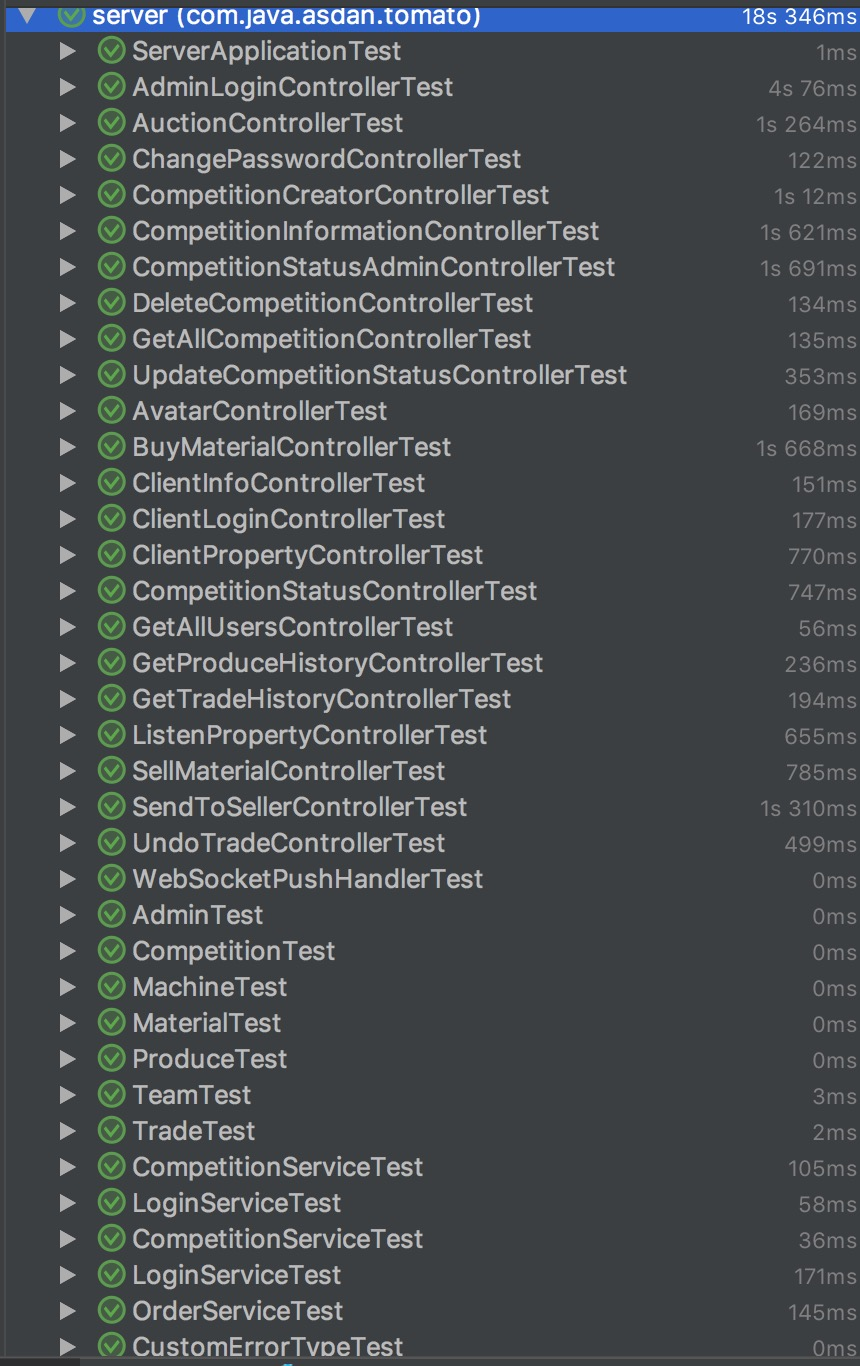
\includegraphics[scale = .3]{fig/test_total_time.jpeg}
		\section{需求的可追踪性}
			本测试计划覆盖了所有后端(除微信WebSocket外)的需求(接口)。
		\section{评价}
			\subsection{评价准则}
				Coverage。
			\subsection{数据处理}
				数据处理由IntelliJ自动完成,IntelliJ将为我们生成完整的Coverage报告。
			\subsection{结论}
				本测试计划十分合理。


\end{document}
